%%%%%%%%%%%%%%%%%%%%%%%%%%%%%%%%%%%%%%%%%%%%%%%%%%%%%%%%%%%%
%%%%% A QUICK INTRODUCTION To LATEX                    %%%%%
%%%%% Philipp Arndt                                    %%%%%
%%%%% UC San Diego, Scripps Instituion of Oceanography %%%%%
%%%%% SIO 115, Ice and the Climate System              %%%%%
%%%%% Winter Quarter 2020                              %%%%%
%%%%%%%%%%%%%%%%%%%%%%%%%%%%%%%%%%%%%%%%%%%%%%%%%%%%%%%%%%%%

% First, we are loading the general settings for the document, which are saved in the file SIOpset.cls. 
\documentclass[letterus,times]{SIOpset}

% Here we can load extra packages, if we need any specific commands
\usepackage{amsmath,mathtools} % American Mathematical Society package
\usepackage{natbib} % a package for managing references

%%%%%%%%%%%%%%%%%%%%%%%%%%%%%%%%%%%%%%%%%%%%%%%%%%%%%%%%%%%%%%%%%%
%%% start document: header
%%%%%%%%%%%%%%%%%%%%%%%%%%%%%%%%%%%%%%%%%%%%%%%%%%%%%%%%%%%%%%%%%%
\begin{document}
 
% IN A HOMEWORK, YOU WOULD SUBSTITUTE YOUR NAME BELOW
% this makes sure your name shows up on every page
\runninghead{Philipp Arndt, SIO 115 Winter 2020, Getting Started with \LaTeX}

% below is our document title
\title{Getting started with \LaTeX}

% IF YOU'RE WRITING UP A DOCUMENT, SUBSTITUTE YOUR OWN NAME BELOW
% this is the author information on the title page
\author{Philipp Arndt\affilnum{1}}

% this is just for the header, you won't have to change anything here if using this for class
\thisquarter{Winter 2020}
\coursenumber{Course: SIO 115}
\coursename{\emph{Ice and the Climate System}}
\instructor{Professor: Helen A. Fricker}

% ADD YOUR MAJOR / DEPARTMENT
\affiliation{%
\affilnum{1}Scripps Polar Center\\
Scripps Institution of Oceanography\\
UC San Diego\\
La Jolla, CA
}

% HERE YOU CAN ADD YOUR PREFERRED EMAIL ADDRESS
\corrauth{\href{mailto:parndt@ucsd.edu}{parndt@ucsd.edu}}

% if you write a paper, you may want to include an abstract
\abstracttitle{Abstract}
\begin{abstract}
Hi, I am an abstract. An abstract should concisely summarize the most important contents of a document. This document provides a template that you may use to submit class-related documents using \LaTeX. It gives a quick introduction and includes some commands that are frequently used. You probably won't need most of these commands, but if you feel stuck somewhere come back to this document! 
\end{abstract}
 
% this command actually compiles the title
\maketitle

% these are some random settings, don't worry about them!
\allowdisplaybreaks
\hypersetup{colorlinks=true, linkcolor=blue}
\renewcommand\thesubsection{\thesection\alph{subsection}}
\renewcommand\thesubsubsection{\thesection\alph{subsection}.\roman{subsubsection}}
\setcounter{secnumdepth}{3} %for section numbering

%%%%%%%%%%%%%%%%%%%%%%%%%%%%%%%%%%%%%%%%%%%%%%%%%%%%%%%%%%%%%%%%%%
% LET'S GET STARTED WITH THE ACTUAL TEXT!!!
%%%%%%%%%%%%%%%%%%%%%%%%%%%%%%%%%%%%%%%%%%%%%%%%%%%%%%%%%%%%%%%%%%

% This section explains how to open a LaTeX template in Overleaf.
% You don't need to worry about the code here, just read the section.
\section{Copy and edit a template on overleaf}
To edit a template on overleaf, you will first need to create an account on \url{https://www.overleaf.com/register} with your email. 
It's free! 
You can then open a read-only link (for this document it's \url{https://www.overleaf.com/read/sfcrvfrbgwhr}) in your browser. 
Just click the 

\includegraphics[width=0.07\textwidth]{figs/intro-menu.png} 
button, and if you are logged in, you have the option to copy the project.

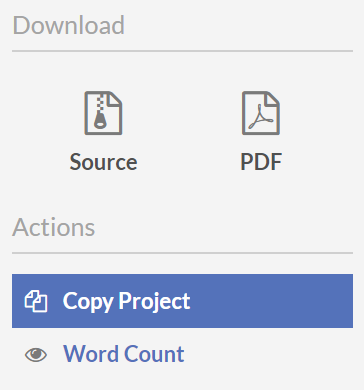
\includegraphics[width=0.2\textwidth]{figs/intro-copy-a-project.png}

Now, you can choose a name for your project.

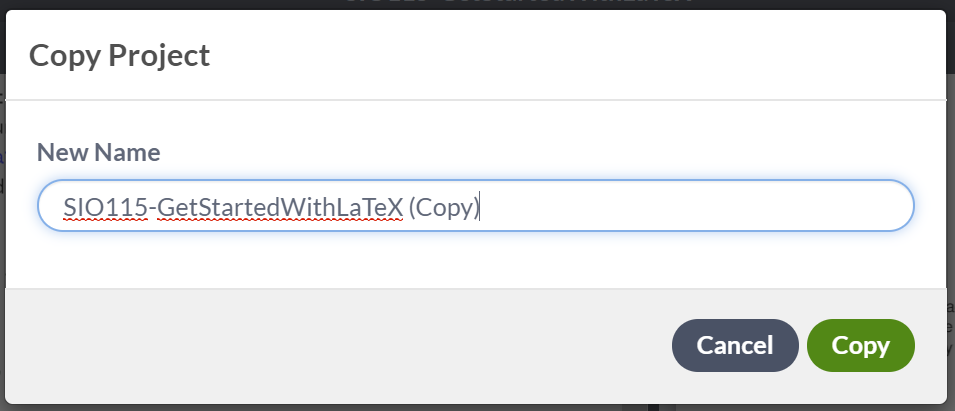
\includegraphics[width=0.35\textwidth]{figs/intro-copy-new-name.png}

If you are working on a homework, I'd recommend naming the file
\texttt{SIO115-HwXX-Lastname-Firstname}, so your document is easily identifiable and already has the right file name when you download it. 
Once you click ``Copy'', you can find your project at \url{https://www.overleaf.com/project}. 
Just click on it, and you're ready to make edits. 

% This section explains how to submit homeworks.
% Again, you don't need to worry about the code here, just read the section.
\section{Homework submission guidelines}

\red{You are expected to submit homework typed up in a \texttt{.pdf} document for this class.} 
Since typing up mathematical equations can be quite a challenge in common text editors such as Microsoft Word, most scientists use \LaTeX\ for this. 
You are allowed to use any program to type up your answers, but encouraged to use \LaTeX! 
To facilitate the use of \LaTeX, you will find templates for each homework on the \href{http://glaciology.weebly.com/timetable.html}{course website}, which are pre-populated with the questions for that homework. 
All that's left for you to do is going to the \texttt{main.tex} document on the directory on the left, adding your own name to the document, and writing your answers wherever it says \emph{``Your answer here.''}. 
For some advice on how to type up mathematical equations, consult section \ref{sec:howToTypeMath}.

Once you are done writing up your answers, you can download the final PDF by clicking the Menu button, and then ``Download PDF''.
When submitting homework, please stick to the naming convention \texttt{SIO115-HwXX-Lastname-Firstname.pdf}, so for example \texttt{SIO115-Hw01-Doe-Jane.pdf} for the first homework.
Please email your answers to \href{mailto:parndt@ucsd.edu}{parndt@ucsd.edu} with subject line \textbf{SIO115 Homework X Lastname Firstname} by the appropriate deadline.

%%%%%%%%%%%%%%%%%%%%%%%%%%%%%%%%%%%%%%%%%%%%%%%%%%%%%%%%%%%%%%%%%%
% FROM HERE ON, THE DOCUMENT SHOWS HOW TO USE SOME BASIC LATEX 
% COMMANDS. HAVE A LOOK AT THE CODE, AND SEE WHAT IT DOES IN THE
% COMPILED PDF DOCUMENT. 
%%%%%%%%%%%%%%%%%%%%%%%%%%%%%%%%%%%%%%%%%%%%%%%%%%%%%%%%%%%%%%%%%%

\section{Some useful \LaTeX\ syntax}
The following sections will introduce some useful commands you can use in \LaTeX\. 
You probably won't need most of these when writing up homework, but it is useful to know some of the things that you could do here. 
Have a look at both the code from here on, and how it shows up in the compiled PDF. 
If there is something else you would want to do, google is usually pretty good at finding the appropriate commands. 
Also, if you need the command for a specific symbol, the app \href{http://detexify.kirelabs.org/classify.html}{detexify} can come in pretty handy. 
Just hand-draw a symbol and it will (most often) find the right command!
If a command requires a specific package, just make sure to load that package at the top of this file with the \verb|\includepackage{}| command.
Also, if you are really stuck with something, I'm happy to help. Just talk to me after class or shoot me an email at \href{mailto:parndt@ucsd.edu}{parndt@ucsd.edu}.

% You can have sections, subsections, etc. that get automtically numbered
\section{I'm a section that demonstrates how to create sections!}
I'm text in this section.
\subsection{I'm a subsection}
I'm text in this subsection.
\subsubsection{I'm a subsubsection}
I'm text in this subsubsection.

% here's a few options to format text
\section{Formatting standard text}
Writing standard text in \LaTeX\ is easy! You can \emph{emphasize} single words or \emph{longer passages of text}, write them in \textbf{bold} or \underline{underline important things}!

Start a new paragraph by simply leaving one line blank. \LaTeX\ will try to automatically figure out how to format your document so that paragraphs aren't broken up in any ``weird-looking'' way. 
If you want to force a new line, you can of course do \\ that as well.

You can also write text in different sizes, such as:

{\Huge Huge}\\
{\huge huge}\\
{\LARGE LARGE}\\
{\Large Large}\\
{\large large} \\
{\normalsize normalsize (default)}\\
{\small small}\\
{\footnotesize footnotesize}\\
{\scriptsize scriptsize}\\
{\tiny tiny}

If you want to change \textcolor{red}{the} \textcolor{green}{color} \textcolor{blue}{of} \textcolor{magenta}{text}, or want to \colorbox{BurntOrange}{highlight} a passage, that also works!

You can include itemized lists with soemthing like this:
\begin{verbatim}
\begin{itemize}
    \item an item
    \item another item
    \item one more item
\end{itemize}
\end{verbatim}
which gives 
\begin{itemize}
    \item an item
    \item another item
    \item one more item.
\end{itemize}
You can do the same with the \verb|enumerate| environment to get numbered lists:
\begin{enumerate}
    \item first item
    \item second item
    \item third item.
\end{enumerate}

If you want to include a link to something on the web, you can do it with the \verb|\url{}| command, like the link to the Scripps Polar Center webpage: \url{https://polar.center/}. 
You can also add a hyperlink to any passage of text with the \verb|\href{}{}| command, like \href{http://glaciology.weebly.com/}{this link} to the Scripps Glaciology group. 

Oh, yeah, and as a little bonus, this template also allows you to use emoji! If you're curious about how that works, just take a look in the \texttt{emojiCommands.sty} file! \thumb \graduation

% if you need to insert a figure or image, look no further!
\section{Adding images or figures and tables}

If you need to include an image, a plot or a drawing in latex, you can do so with the \verb|\includegraphics[]{}| command. 
Usually it makes sense to include this in a figure environment like this:
\begin{verbatim}
\begin{figure}
    \centering
    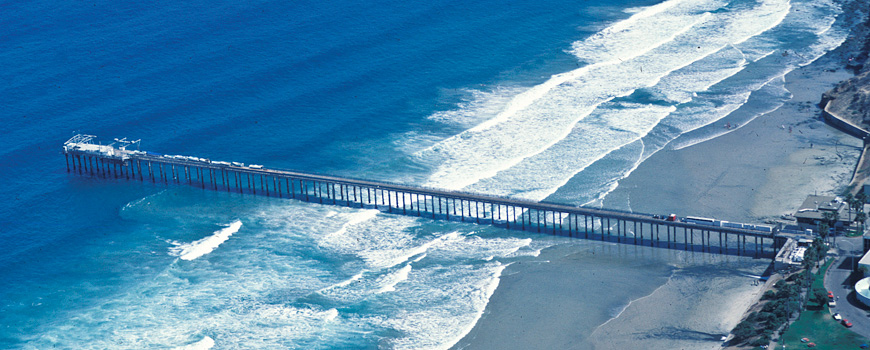
\includegraphics[width=0.48\textwidth]
    {figs/scripps-pier.jpg}
    \caption{A great place to study ice and 
    snow.}
    \label{fig:my_figure}
\end{figure}
\end{verbatim}
\begin{figure}
    \centering
    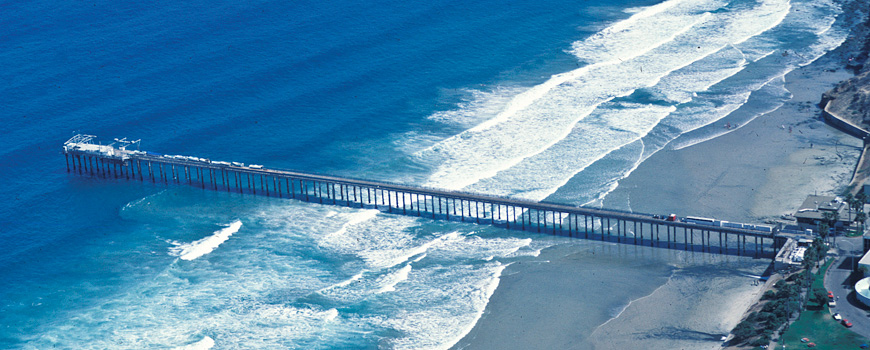
\includegraphics[width=0.48\textwidth]{figs/scripps-pier.jpg}
    \caption{A great place to study ice and snow.}
    \label{fig:my_figure}
\end{figure}
\LaTeX\ now places the figure at a (most of the time) convenient location in the text, and you can refer to it with the \verb|\ref{}| command like this (see figure \ref{fig:my_figure}).

Similarly, you can add tables with the \verb|tabular| environment like shown in table \ref{tab:applesnoranges}.
\begin{table}[h]
\centering
\begin{tabular}{||l | c | c||}
\hline Person   & Apples & Oranges\\[0.2ex] 
 \hline\hline
\hline Anne & 3 & 5 \\
\hline Peter & 4 & 7\\
\hline Taylor & 12 & 0\\ \hline 
\end{tabular}
\caption{\vspace{0.2cm} Distribution of fruit.}
\label{tab:applesnoranges}
\end{table}

% now the real stuff: typing up math-y things!
\section{Typing Math / Equations} \label{sec:howToTypeMath}

\subsection{Inline math}
If you want to type math inline, you need to use dollar signs like this \verb|$a^2 + b^2 = c^2$|, which will give you $a^2 + b^2 = c^2$.
You can use Greek letters by using a backslash, followed by the name of the letter. This way, the command \verb|$\alpha \beta \gamma \delta \Gamma \Delta$|
gives $\alpha \beta \gamma \delta \Gamma \Delta$.

\subsection{Subscripts and superscripts}
Superscripts can be typed using \verb|^| and subscripts use \verb|_|. This way 
\begin{itemize}
    \item \verb|$a^2$| becomes $a^2$
    \item \verb|$b_i$| becomes $b_i$, and
    \item \verb|$c_{ij}^{12}$| becomes $c_{ij}^{12}$.
\end{itemize}

\subsection{Equations in display mode}
If you want to write longer equations, you may want to highlight them by giving them their own line. For this you can use the \verb|equation| environment:
\begin{equation} \label{eq:pythagoras}
    a^2 + b^2 = c^2
\end{equation}
Note here that the equation is numbered. You can now refer back to that equation in the text. Here, the Pythagorean Theorem is shown in equation \ref{eq:pythagoras}.
If you don't need the numbering, you can suppress it by using the \verb|equation*| environment like this: 
\begin{equation*}
    \norm{\avg{\bm u, \bm v}}^2 \leq \avg{\bm u, \bm u} \cdot \avg{\bm v, \bm v}
\end{equation*}

\subsection{Some useful math symbols and commands}
\begin{tabular}{|| c | c||}
\hline command   & symbol\\[0.2ex] 
 \hline\hline
\hline \verb|\leq| & $\leq$\\
\hline \verb|\geq| & $\geq$\\
\hline \verb|\neq| & $\neq$\\
\hline \verb|\approx| & $\approx$\\
\hline \verb|\partial| & $\partial$\\
\hline \verb|\cdot| & $\cdot$\\
\hline \verb|\times| & $\times$\\
\hline \verb|\ldots| & $\ldots$\\
\hline \verb|\forall| & $\forall$\\
\hline \verb|\in| & $\in$\\
\hline \verb|\exists| & $\exists$\\
\hline \verb|\infty| & $\infty$\\
\hline \verb|\sqrt{x}| & $\sqrt{x}$\\
\hline \verb|\sum| & $\sum$\\
\hline \verb|\sum_{i=0}^{10} i| & $\sum_{i=0}^{10} i$\\
\hline \verb|\int| & $\int$\\
\hline \verb|\int_{0}^{2\pi} \sin{x}\ dx| & $\int_{0}^{2\pi} \sin{x}\ dx$\\
\hline \verb|\frac{x}{y}| & $\frac{x}{y}$\\
\hline \verb|\frac{\text{this}}{\text{that}}| & $\frac{\text{this}}{\text{that}}$\\
\hline \verb|\left(\frac{x}{y}\right)| & $\left(\frac{x}{y}\right)$\\
\hline 
\end{tabular}

\subsection{Aligning equations}
If you make calculations with multiple steps, you may want to align your math at the equal sign for each step. This is achieved with the \verb|align| (or \verb|align*|) environment. Just add a \verb|&| wherever you want to align the equation, and use \verb|\\| to break the line. 
\begin{align*}
    \left(a + b\right)^2 &= (a + b) (a + b) \\
    &= a\times a + a\times b + b\times a + b\times b \\
    &= a^2 + 2ab + b^2
\end{align*}

% don't plagiarize and include your sources if you used any!
\section{Referencing sources}

To cite any sources you may have used, you need to save all your references in a format called BibTeX. In this template, all the references are saved in the file \texttt{lit.bib}. The bibtex code for the textbook, for example is 
\begin{verbatim}
@book{marshall2011cryosphere,
  title={The cryosphere},
  author={Marshall, Shawn J},
  volume={2},
  year={2011},
  publisher={Princeton University Press}
}
\end{verbatim}
The good news is that for any book or paper that you can find on Google Scholar, you can just hit the 
\includegraphics[scale=0.8]{figs/cite.png} icon and then ``BibTeX''. This gives you the BibTeX code that you can copy-paste directly into your bibliography file. 
Now, you can cite that this book with the \verb|\citep{}| command, using the identifier in the first line of the BibTeX code \citep{marshall2011cryosphere}. 
You can also reference a paper such as \cite{fricker2007active} without the parentheses using the \verb|\cite{}| command. 
If you want to include a source in the reference list, but don't mention it in your text, you can do that with the \verb|\nocite{}| command. 
\nocite{holton2004} % this one doesn't appear in the text, but check out the reference list
Now, all you need to do to generate your list of references is to call your bibliography file with the \verb|\bibliography{}| command! % see right below

%%%%%%%%%%%%%%%%%%%%%%%%%%%%%%%%%%%%%%%%%%%%%%%%%%%%%%%%%%%%%%%%%%
%%% BIBLIOGRAPHY
%%%%%%%%%%%%%%%%%%%%%%%%%%%%%%%%%%%%%%%%%%%%%%%%%%%%%%%%%%%%%%%%%%
\setcitestyle{numbers} % use this to include numbers
\bibliographystyle{plainnat} % use this to set the citation style
\bibliography{lit.bib} % UNCOMMENT THIS LINE IF NO REFERENCES NEEDED


%%%%%%%%%%%%%%%%%%%%%%%%%%%%%%%%%%%%%%%%%%%%%%%%%%%%%%%%%%%%%%%%%%
%%% CODE SUBMISSION (if needed...)
%%%%%%%%%%%%%%%%%%%%%%%%%%%%%%%%%%%%%%%%%%%%%%%%%%%%%%%%%%%%%%%%%%

% \electronicfalse % COMMENT OUT TO SUBMIT CODE

\ifelectronic 
\section{Appendix: How to include files of code}

% EXAMPLE FOR GENERIC NON-HIGHLIGHTED CODE
You can load any code from a text file like this:
\codeexternal{code/myCode.cpp} % enter code file name here

% EXAMPLE FOR MATLAB
Other commands in this template allow you to use highlighting for Matlab...
\matlabexternal{code/myCode.m} % enter code file name here

% EXAMPLE FOR Python
...or Python!
\pythonexternal{code/myCode.py} % enter code file name here

\fi % end code submission

%%%%%%%%%%%%%%%%%%%%%%%%%%%%%%%%%%%%%%%%%%%%%%%%%%%%%%%%%%%%%%%%%%
\end{document}
%%%%%%%%%%%%%%%%%%%%%%%%%%%%%%%%%%%%%%%%%%%%%%%%%%%%%%%%%%%%%%%%%%
